\documentclass{beamer}

\usepackage{algorithm}
\usepackage{algpseudocode}
\usepackage{mathtools}

\usefonttheme{serif}
\usepackage{dsfont}
\setbeamersize{text margin left=5pt, text margin right=5pt}

\newcommand{\bgk}[1]{\boldsymbol{#1}}

\newcommand{\bzero}{\bgk{0}}
\newcommand{\bone}{\bgk{1}}

\newcommand{\balpha}{\bgk{\alpha}}
\newcommand{\bnu}{\bgk{\nu}}
\newcommand{\bbeta}{\bgk{\beta}}
\newcommand{\bxi}{\bgk{\xi}}
\newcommand{\bgamma}{\bgk{\gamma}} 
\newcommand{\bo}{\bgk{o }}
\newcommand{\bdelta}{\bgk{\delta}}
\newcommand{\bpi}{\bgk{\pi}}
\newcommand{\bepsilon}{\bgk{\epsilon}} 
\newcommand{\bvarepsilon}{\bgk{\varepsilon}} 
\newcommand{\brho}{\bgk{\rho}}
\newcommand{\bvarrho}{\bgk{\varrho}}
\newcommand{\bzeta}{\bgk{\zeta}}
\newcommand{\bsigma}{\bgk{\sigma}}
\newcommand{\boldeta}{\bgk{\eta}}
\newcommand{\btay}{\bgk{\tau}}
\newcommand{\btheta}{\bgk{\theta}}
\newcommand{\bvertheta}{\bgk{\vartheta}}
\newcommand{\bupsilon}{\bgk{\upsilon}}
\newcommand{\biota}{\bgk{\iota}}
\newcommand{\bphi}{\bgk{\phi}}
\newcommand{\bvarphi}{\bgk{\varphi}}
\newcommand{\bkappa}{\bgk{\kappa}}
\newcommand{\bchi}{\bgk{\chi}}
\newcommand{\blambda}{\bgk{\lambda}}
\newcommand{\bpsi}{\bgk{\psi}}
\newcommand{\bmu}{\bgk{\mu}}
\newcommand{\bomega}{\bgk{\omega}}

\newcommand{\bA}{\bgk{A}}
\newcommand{\bDelta}{\bgk{\Delta}}
\newcommand{\bLambda}{\bgk{\Lambda}}
\newcommand{\bSigma}{\bgk{\Sigma}}
\newcommand{\bOmega}{\bgk{\Omega}}
\newcommand{\bPsi}{\bgk{\Psi}}

\newcommand{\bvec}[1]{\mathbf{#1}}

\newcommand{\va}{\bvec{a}}
\newcommand{\vb}{\bvec{b}}
\newcommand{\vc}{\bvec{c}}
\newcommand{\vd}{\bvec{d}}
\newcommand{\ve}{\bvec{e}}
\newcommand{\vf}{\bvec{f}}
\newcommand{\vg}{\bvec{g}}
\newcommand{\vh}{\bvec{h}}
\newcommand{\vi}{\bvec{i}}
\newcommand{\vj}{\bvec{j}}
\newcommand{\vk}{\bvec{k}}
\newcommand{\vl}{\bvec{l}}
\newcommand{\vm}{\bvec{m}}
\newcommand{\vn}{\bvec{n}}
\newcommand{\vo}{\bvec{o}}
\newcommand{\vp}{\bvec{p}}
\newcommand{\vq}{\bvec{q}}
\newcommand{\vr}{\bvec{r}}
\newcommand{\vs}{\bvec{s}}
\newcommand{\vt}{\bvec{t}}
\newcommand{\vu}{\bvec{u}}
\newcommand{\vv}{\bvec{v}}
\newcommand{\vw}{\bvec{w}}
\newcommand{\vx}{\bvec{x}}
\newcommand{\vy}{\bvec{y}}
\newcommand{\vz}{\bvec{z}}

\newcommand{\vA}{\bvec{A}}
\newcommand{\vB}{\bvec{B}}
\newcommand{\vC}{\bvec{C}}
\newcommand{\vD}{\bvec{D}}
\newcommand{\vE}{\bvec{E}}
\newcommand{\vF}{\bvec{F}}
\newcommand{\vG}{\bvec{G}}
\newcommand{\vH}{\bvec{H}}
\newcommand{\vI}{\bvec{I}}
\newcommand{\vJ}{\bvec{J}}
\newcommand{\vK}{\bvec{K}}
\newcommand{\vL}{\bvec{L}}
\newcommand{\vM}{\bvec{M}}
\newcommand{\vN}{\bvec{N}}
\newcommand{\vO}{\bvec{O}}
\newcommand{\vP}{\bvec{P}}
\newcommand{\vQ}{\bvec{Q}}
\newcommand{\vR}{\bvec{R}}
\newcommand{\vS}{\bvec{S}}
\newcommand{\vT}{\bvec{T}}
\newcommand{\vU}{\bvec{U}}
\newcommand{\vV}{\bvec{V}}
\newcommand{\vW}{\bvec{W}}
\newcommand{\vX}{\bvec{X}}
\newcommand{\vY}{\bvec{Y}}
\newcommand{\vZ}{\bvec{Z}}

\usepackage{subcaption}
\newcommand{\bitem}{\item[$\bullet$]}

\usepackage{xcolor}
\usepackage[utf8]{inputenc}
\DeclareFontEncoding{LS1}{}{}
\DeclareFontSubstitution{LS1}{stix}{m}{n}
\DeclareSymbolFont{symbols2}{LS1}{stixfrak} {m} {n}
\DeclareMathSymbol{\operp}{\mathbin}{symbols2}{"A8}
\setbeamertemplate{navigation symbols}{}

\usepackage{lipsum}

\newtheorem{proposition}[theorem]{Proposition}

\newcommand\blfootnote[1]{%
  \begingroup
  \renewcommand\thefootnote{}\footnote{#1}%
  \addtocounter{footnote}{-1}%
  \endgroup
}

\addtobeamertemplate{navigation symbols}{}{%
    \usebeamerfont{footline}%
    \usebeamercolor[fg]{footline}%
    \hspace{1em}%
    \insertframenumber/\inserttotalframenumber
}

\title{
Krylov Subspace Methods\\ -- Linear Systems -- \\
Lecture 22
}
%\subtitle{Mathematical framework, existence and exactness}

\author{F. M. Faulstich}
\date{04/16/2024}

\begin{document}

\frame{\titlepage}


\begin{frame}{Krylov Subspace Methods}

\begin{itemize}
    \bitem Depending on the problem different names arise\\
    ~\\
    \begin{figure}
        \centering
        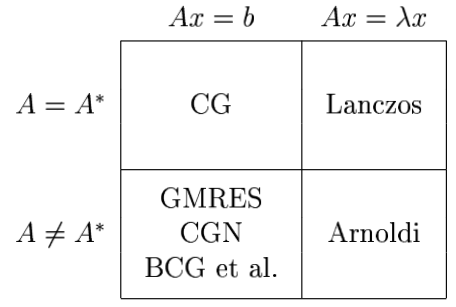
\includegraphics[width=.5\textwidth]{Graphics/KrylovMethods.png}
    \end{figure}
\end{itemize}
    
\end{frame}

\begin{frame}{Quadratic Test function}

\begin{itemize}
    \bitem Consider the {\it quadratic test function}:\\
    Let $0 \prec \vA \in\mathbb{R}^{n \times n} $ and $\vb,\vx \in \mathbb{R}^n$
    $$
    \phi(\vx) = \frac{1}{2}\vx^\top \vA \vx - \vx^\top \vb
    $$
    \bitem The gradient of $\phi$ is given by
    $$
    \nabla \phi (\vx)
    =
    \vA\vx - \vb
    $$
    Hence, at the critical point $\vx_*$ we have
    $$
    \nabla \phi (\vx_*) = 0 \quad \Leftrightarrow \quad \vA \vx_* = \vb
    $$
    \bitem Is this critical point unique? -- Yes!
    \begin{itemize}
        \item[i)] Note that 
        $$
        \nabla^2 \phi(\vx)= \vA \succ \bzero
        $$
        $\Rightarrow$ $\vx_*$ is a minimum
        \item[ii)] $\nabla^2 \phi(\vx)$ is constant! $\Rightarrow$ $\phi$ is convex.
    \end{itemize}
\end{itemize}
    
\end{frame}

\begin{frame}{Line Search Methods}

\begin{itemize}
    \bitem {\it Line search methods} are iterative optimization method
    \bitem Idea:\\
    Start with an initial guess $\vx_0$\\ 
    Update as
    $$
    \vx_{k+1} = \vx_k + \alpha_k \vp_k
    $$
    where $\vp_k$ is the {\it search direction}
    and $\alpha_k$ is the {\it step length}
\end{itemize}
    
\end{frame}

\begin{frame}{Steepest Descent}

\begin{itemize}
    \bitem Remember
    $$
    \nabla \phi (\vx)
    =
    \vA\vx - \vb
    $$
    points towards largest increase of $\phi$ in $\vx$.\\
    $\Rightarrow$ Search direction should be $\vp_k = - \nabla \phi (\vx_k) = \vr(\vx_k)$
    \bitem What about the step length?\\
    Idea: Walk until we no longer descend!
    $$
    0 \overset{!}{=} \partial_{\alpha_k} \phi(\vx_{k+1})
    \quad \Rightarrow \quad 
    \alpha_k
    =
    \frac{\vr_k^\top \vr_k}{\vr_k^\top \vA \vr_k}
    $$
\end{itemize}
    
\end{frame}

\begin{frame}{Convergence}

\begin{figure}
    \centering
    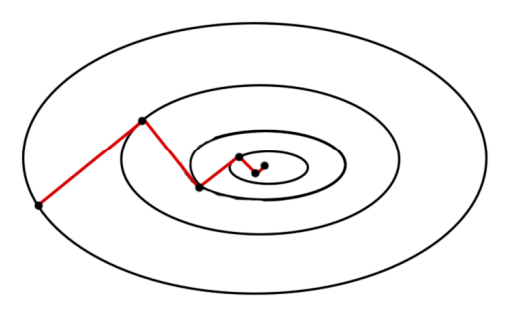
\includegraphics[width = .5\textwidth]{Graphics/StepestDescendConv.png}
\end{figure}

\begin{center}
$\Rightarrow$ ``ZigZag'' convergence cannot be optimal!
\end{center}
~\\
Question: Can we use information from the previous iterations?
\end{frame}


\begin{frame}{$\vA$-conjugate direction}

\begin{itemize}
    \bitem We say a set of vectors $\{\vp_1,...,\vp_{k}\}$ are conjugate w.r.t. the SPD matrix $\vA$ iff
    $$
    \vp_i^\top \vA \vp_j = 0 \quad \forall i \neq j 
    $$
    \bitem Claim: $n$ $\vA$-conjugate vectors form a basis of $\mathbb{R}^n$.
    \bitem Then
    $$
    \vx_*
    =
    \sum_{i=1}^{n} c_i\vp_i 
    \quad \Rightarrow \quad
    \vA\vx_*
    = \sum_{i=1}^{n} c_i \vA \vp_i 
    $$
    hence
    $$
    \vp_k^\top\vb
    =
    \sum_{i=0}^{n-1} c_i \vp_k^\top \vA \vp_i
    =
    c_k \vp_k^\top \vA \vp_k
    \quad \Rightarrow \quad
    c_k = \frac{\vp_k^\top\vb}{\vp_k^\top \vA \vp_k}
    $$
    \bitem If we have sequence of $\vA$-conjugate vecorts we can solve for $\vx_*$
\end{itemize}
    
\end{frame}

\begin{frame}{$\vA$-conjugate vectors}

\only<1>{
\begin{center}
How do we find the set of $\vA$-conjugate vectors?
\end{center}
}

\only<2>{
Zeroth Iteration:
\begin{itemize}
    \bitem We start with $\vx_0 = \bzero\in\mathbb{R}^n$
    \bitem Compute the residual 
    $$
    \vr_0 = \vb - \vA \vx_0
    $$
    \bitem Compute the search direction
    $$
    \vp_0 = -\nabla \phi(\vx_0) = \vr_0
    $$
    \bitem Compute the step length
    $$
    \alpha_0 = \frac{\vp_0^\top \vr_0}{\vp_0^\top \vA \vp_0}
    $$
    \bitem Update the iterate
    $$
    \vx_1 = \vx_0 + \alpha_0 \vp_0
    $$
    
\end{itemize}
}

\only<3>{
k$th$ iteration:
\begin{itemize}
    \bitem Compute the residual 
    $$
    \vr_k = \vb - \vA \vx_k = -\nabla \phi(\vx_k)
    $$
    \bitem Make the gradient conjugate to the previous $\{\vp_0,...,\vp_{k-1}\}$
    $$
    \vp_k
    =
    \vr_k - \sum_{i=0}^{k-1}\frac{\vp_i^\top \vA \vr_k}{\vp_i^\top \vA \vp_i}\vp_i
    $$
    \bitem Compute the step length
    $$
    \alpha_k = \frac{\vp_k^\top \vr_k}{\vp_k^\top \vA \vp_k}
    $$
    \bitem Update the iterate
    $$
    \vx_{k+1} = \vx_k + \alpha_k \vp_k
    $$
\end{itemize}

}

\end{frame}

\begin{frame}{Computation of the search direction}

\begin{itemize}
\begin{footnotesize}
    \bitem Let's take a closer look at the search direction
    $$
    \vp_k
    =
    \vr_k - \sum_{i=0}^{k-1}\frac{\vp_i^\top \vA \vr_k}{\vp_i^\top \vA \vp_i}\vp_i
    $$
    \bitem Better to impose conjugation explicitly:
    $$
    \vp_k = \vr_k - \beta_k \vp_{k-1}
    $$
    Then $\vp_{k-1}^\top \vA \vp_{k} = 0 $ implies
    $$
    \beta_k = \frac{\vp_{k-1}^\top \vA \vr_{k}}{\vp_{k-1}^\top \vA \vp_{k-1}}
    $$
    Note that
    $$
    \vr_{k}^\top \vA \vp_{k-1} 
    %= \frac{1}{\alpha_{k-1}}\vr_k^\top (\vr_k - \vr_{k-1})
    = -\frac{1}{\alpha_{k-1}}\vr_k^\top \vr_k
    \quad
    {\rm and}
    \quad
    \vp_k^\top \vA \vp_k
    %= (-\vr_k + \beta_{k-1}\vp_{k-1})^\top \vA \vp_k
    = \frac{1}{\alpha_k} \vr_{k}^\top \vr_k
    $$
    Hence
    $$
    \beta_k = -\frac{\vr_k^\top \vr_k}{\vr_{k-1}^\top \vr_{k-1}}
    $$
\end{footnotesize}
\end{itemize}
    
\end{frame}

\begin{frame}{Conjugate Gradient Algorithm}

\begin{itemize}
    \item[] Input: $\vA$\vspace{-2mm}
    \item[] Output: $\vx$ approximate solution to $\vA \vx_* = \vb$
    \item[] $\vx_0 = \bzero$
    \item[] $\vp_0 = \vr_0 = \vb - \vA \vx_0$
    \item[] For k=1...
    \item[] $\quad$ $\alpha_{k-1} = \frac{\vp_{k-1}^\top \vr_{k-1}}{\vp_{k-1}^\top \vA \vp_{k-1}}$
    \item[] $\quad$ $\vx_k = \vx_{k-1} + \alpha_{k-1} \vp_{k-1}$
    \item[] $\quad$ $\vr_k = \vb - \vA \vx_{k}$ 
    \item[] $\quad$ $\beta_k = -\frac{\vr_k^\top \vr_k}{\vr_{k-1}^\top \vr_{k-1}}$
    \item[] $\quad$ $\vp_{k} = \vr_{k} - \beta_k \vp_{k-1}$
\end{itemize}

    
\end{frame}


\begin{frame}{}

\begin{center}
Why is this a Krylov subspace method?
\end{center}
    
\end{frame}


\begin{frame}{}
\begin{itemize}
    \bitem Claim:
$\vx_k\in\mathcal{K}_k = {\rm span}(\vb, \vA\vb,...,\vA^{k-1}\vb)$
    \bitem Claim: $\vr_k \perp \mathcal{K}_k$
\bitem Theorem: \\
$\vx_k\in \mathcal{K}_k$ is the unique point that minimizes $\Vert \ve_k \Vert_A$ with $\ve_k = \vx_* - \vx_k$ and $\Vert \ve_k \Vert\leq \Vert \ve_{k-1} \Vert$ and $\ve_\ell = 0 $ for some $\ell \leq n$.
\end{itemize}
\end{frame}

\end{document}




